%%%%%%%%%%%%%%%%%%%%%%%%%%%%%%%%%%%%%%%%%%%%%%%%%%%%%%%%%%%%%%%%%%%%%%%%%%%%%%%%%%%%%%%%%%%%%%%%%%%%%%%%%%%%%%%%%%%%%%%%%%%%%%%%%%%%%%%%%%%%%%%%%%%%%%%%%%%%%%%%%%%
% Written By Michael Brodskiy
% Class: Circuits & Signals: Biomedical Applications
% Professor: N. Sun
%%%%%%%%%%%%%%%%%%%%%%%%%%%%%%%%%%%%%%%%%%%%%%%%%%%%%%%%%%%%%%%%%%%%%%%%%%%%%%%%%%%%%%%%%%%%%%%%%%%%%%%%%%%%%%%%%%%%%%%%%%%%%%%%%%%%%%%%%%%%%%%%%%%%%%%%%%%%%%%%%%%

\documentclass[12pt]{article} 
\usepackage{alphalph}
\usepackage[utf8]{inputenc}
\usepackage[russian,english]{babel}
\usepackage{titling}
\usepackage{amsmath}
\usepackage{graphicx}
\usepackage{enumitem}
\usepackage{amssymb}
\usepackage[super]{nth}
\usepackage{everysel}
\usepackage{ragged2e}
\usepackage{geometry}
\usepackage{multicol}
\usepackage{fancyhdr}
\usepackage{cancel}
\usepackage{siunitx}
\usepackage{physics}
\usepackage{tikz}
\usepackage{mathdots}
\usepackage{yhmath}
\usepackage{cancel}
\usepackage{color}
\usepackage{array}
\usepackage{multirow}
\usepackage{gensymb}
\usepackage{tabularx}
\usepackage{extarrows}
\usepackage{booktabs}
\usetikzlibrary{fadings}
\usetikzlibrary{patterns}
\usetikzlibrary{shadows.blur}
\usetikzlibrary{shapes}

\geometry{top=1.0in,bottom=1.0in,left=1.0in,right=1.0in}
\newcommand{\subtitle}[1]{%
  \posttitle{%
    \par\end{center}
    \begin{center}\large#1\end{center}
    \vskip0.5em}%

}
\usepackage{hyperref}
\hypersetup{
colorlinks=true,
linkcolor=blue,
filecolor=magenta,      
urlcolor=blue,
citecolor=blue,
}


\title{Operational Amplifiers}
\date{\today}
\author{Michael Brodskiy\\ \small Professor: N. Sun}

\begin{document}

\maketitle

\begin{itemize}

  \item Frequency

    \begin{itemize}

      \item Terminology: $\omega_0$ is the fundamental frequency, $T$ is the period, $n\omega_0$ are harmonics of $\omega_0$ or harmonic frequencies of $f(t)$

        $$a_0=\frac{1}{T}\int_{t_0}^{t_0+T} f(t)\,dt\,\,\,\,\,\,\,\,\text{(This is the average of the signal over a period)}$$
        $$a_n=\frac{2}{T}\int_{t_0}^{t_0+T} f(t)\cos(n\omega_0t)\,dt\,\,\,\,\,\,\,\,\text{(This is how much the signal “looks” like a cos at $k\omega_0$)}$$
        $$b_n=\frac{2}{T}\int_{t_0}^{t_0+T} f(t)\sin(n\omega_0t)\,dt\,\,\,\,\,\,\,\,\text{(This is how much the signal “looks” like a sin at $k\omega_0$)}$$

    \end{itemize}

  \item Amplifiers

    \begin{itemize}

      \item Denoted as a triangle pointed in direction of current in circuit diagrams

      \item A signal is usually represented as current ($i$) or voltage ($v$)

      \item The purpose of amplifier is to increase the magnitude of incoming signal for meaningful use

      \item For example, a loud-speaker increases the amount of sound waves to make it audible to a public gathering

      \item You can increase or decrease the brightness of your computer screen by controlling the amount of amplification of the LED display

      \item The input signal can be ($v$ or $i$) and the output signal can also be amplified version of ($v$ or $i$).

      \item This gives us 4 combinations:

        \begin{enumerate}

          \item A Voltage Amplifier amplifies voltage Input ($v$) to provide a voltage output ($Av$).

          \item A Current Amplifier amplifies current Input ($i$) to provide a current output ($Ai$).

          \item A Transconductance Amplifier amplifies voltage Input ($v$) to provide a current output ($Ai$).

          \item A Transresistance Amplifier amplifies current Input ($i$) to provide a voltage output ($Av$).

        \end{enumerate}

        \begin{itemize}

          \item $A$ is called the gain of the amplifier.

          \item $A$ can be dimensionless or can have the dimension of resistance or conductance.

        \end{itemize}

    \end{itemize}

  \item Operational Amplifiers

    \begin{itemize}

      \item Built out of diodes and transistors

      \item A complex circuit, but we will not study its internal details

      \item It has a very simplified terminal characteristics.

      \item Equivalent model is essentially a circuit with dependent source.

      \item Op-Amps are very common place in electronics systems.

      \item We are only interested in OP-Amp terminal characteristics and not its internal circuitry.

    \end{itemize}

  \item In 1968, Fairchild made a popular Op-Amp which was an 8-pin micro-chip

    \begin{itemize}

      \item Out of 8 terminals, terminals NC and two offset terminals will not be discussed in this class

      \item Essentially, our Op-Amp will be a 5-terminal device

      \item Two input terminals:

        \begin{itemize}

          \item The $+ve$ terminal is called the non-inverting input

          \item The $-ve$ terminal is called the inverting input

        \end{itemize}

      \item One output terminal

      \item Two power supplies, a $+ve$ voltage and a $-ve$ voltage

    \end{itemize}

  \item The Op-Amp Operating Region

    \begin{itemize}

      \item The input voltage to the Op-Amp is $v_i=(v_p-v_n)$

      \item The output voltage of the Op-Amp is $Av_i=A(v_p-v_n)$

      \item The Op-Amp output has two regions: linear and saturation, as defined below

        $$v_0=\left\{\begin{array}{l l}-V_{CC} & A(v_p-v_n) < -V_{CC},\\A(v_p-v_n) & -V_{CC} \leq A(v_p-v_n) \leq +V_{CC},\\ +V_{CC} & A(v_p-v_n) > +V_{CC}  \end{array}$$

    \end{itemize}

  \item Op-Amp Gain

    \begin{itemize}
        
      \item In practical applications, Op-Amps are rarely used in an open-loop configuration

      \item It is almost always used in a feedback configuration

      \item Feedback is when output is connected back to an input using circuit components

      \item When it is connected to the negative terminal, it is called negative feedback, and for the positive terminal, it is called positive feedback

    \end{itemize}

    \begin{figure}[h!]
      \centering
      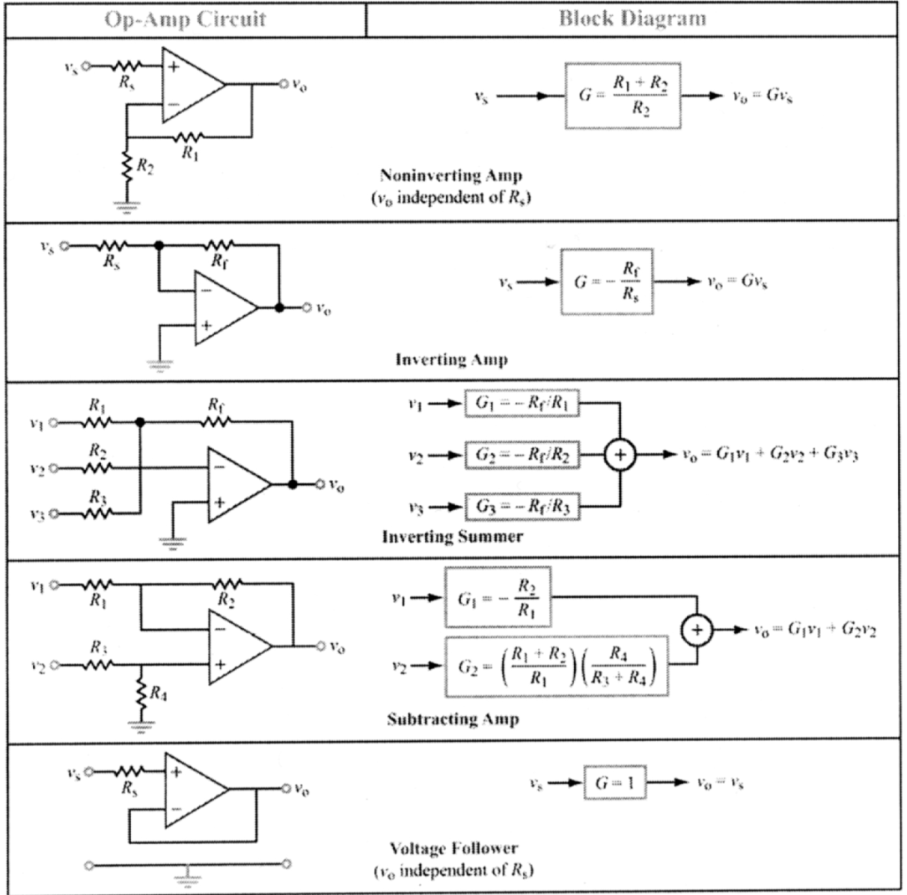
\includegraphics[width=.9\textwidth]{Figures/OPAMPS.png}
      \caption{OpAmp Shortcuts}
      \label{fig:1}
    \end{figure}

\end{itemize}

\end{document}

